\chapter{Exposure Assessment and Dosimetry in the Era of 5G}
\label{chap:methods}

\section{Specific Absorption Rate}
Generally, heating effects are correlated well with the amount of \gls{em} field power absorbed by biological tissue.
The total power absorbed per unit mass is given in terms of \gls{sar} which is measured in \SI{}{\watt\per\kg}.
According to~\cite{Foster2022Three}, the first mention of the term ``\gls{sar}'' is found in 1975 PhD dissertation by Chou~\cite{Chou1975Effects}.

Mathematically, \gls{sar} represents the rate of change at which \gls{em} energy is absorbed by or dissipated in a unit mass, contained in a volume element:
\begin{align}
    \label{eqn:sar_1}
    \text{SAR} = \frac{\partial}{\partial t} \Big( \frac{\partial W}{\partial m} \Big).
\end{align}
If exposed tissue has a constant density, $\rho$, the above expression can be written as
\begin{align}
    \label{eqn:sar_2}
    \text{SAR} = \frac{\partial}{\partial t} \Big( \frac{\partial W}{\rho \; \partial V} \Big),
\end{align}
where $V$ is a volume element of interest.
In dielectric sense, any biological tissue can be described as lossy, magnetically transparent material characterized by the frequency dependent relative complex dielectric permittivity,  $\varepsilon^*$, and relative permeability, $\mu_r = 1$~\cite{Sasaki2014Measurement}.
Therefore, in practical situations, \gls{sar} can be assessed by using the following expression:
\begin{align}
    \label{eqn:sar_3}
    \text{SAR} = \frac{\sigma \; |\mathbf{E}|^2}{\rho},
\end{align}
where $\sigma$ represents the conductivity of tissue measured in \SI{}{\siemens\per\m}, and $\mathbf{E}$ is the \gls{rms} value of the electric field at a single point within tissue.

Temperature rise of the exposed tissue is shown to be strongly correlated with the value of \gls{sar}, and in the case of brief \gls{em} exposure where heat loss is not significant, it can be approximated as
\begin{align}
    \label{eqn:sar_4}
    \text{SAR} = C \; \frac{\partial T}{\partial t},
\end{align}
where $C$ is specific heat capacity expressed in \SI{}{\joule\per\kg\per\celsius}, and $T$ is temperature in \SI{}{\celsius}.
However, in realistic exposure scenarios that are neither brief nor can be treated by homogeneous models, heat loss is significant as a large amount of heat rapidly diffuses due to active thermoregulatory mechanism.
For this reason, \gls{sar}, as a proxy for temperature rise, must be averaged over either whole body, or, in the case of local exposure, 10-g equivalent of tissue volume~\cite{McIntosh2011SAR}.
Spatially-averaged \gls{sar} over \SI{10}{g} has been shown to approximate temperature rise well up to \SI{6}{\GHz} for both the homogeneous cubical and morphologically accurate body model~\cite{Hirata2009correlation}.
Additionally, in cases where simplistic tissue models are utilized, peak-spatial \gls{sar} can also be used to correlate temperature rise at lower frequencies, concretely \SI{150}{}, \SI{400}{} and \SI{900}{\MHz} bands, which is confirmed by considering a 3-D realistic human body model~\cite{Hirata2006Correlation}.
At higher frequencies, especially above \SI{6}{\GHz}, the same cannot be stated as the correlation between peak-spatial \gls{sar} and maximum temperature rise is at most modest for realistic exposure of morphologically accurate body models~\cite{Morimoto2016Relationship}.

Whole-body exposure is accompanied with the assessment of whole-body average \gls{sar}, which is dependent on the spatial distribution of the internal electric field, electric conductivity of tissue, and tissue density.
Taking all this into account, whole-body averaged \gls{sar} is defined as the ratio of the total power absorbed in the whole body and the whole body mass:
\begin{align}
    \label{eqn:sar_wb}
    \text{whole-body SAR} = \frac{\int_{V_\text{wb}} \sigma \; |\mathbf{E}|^2 \; \mathrm{d}V}{\int_{V_\text{wb}} \rho \; \mathrm{d}V},
\end{align}
where $V_\text{wb}$ is the volume of the exposed body.

Different averaging schemes and masses have been numerically analyzed in terms of how well they predict local temperature rise~\cite{Hirata2009correlation,McIntosh2011SAR}.
It is generally accepted that a cubic averaging mass of \SI{10}{\g}, including all tissues, serves as an appropriate spatial averaging volume equivalent up to \SI{6}{\GHz}.
Furthermore, it is important to note that 10-g volume corresponds to approximately \SI{2.15}{\cm\cubed} cube assuming that the density of exposed tissue is the same as that of water, i.e., \SI{1000}{\kg\per\m\cubed}.

On average, the time required to reach a steady state for the case of the whole body exposure is 30 minutes or more, while for the local exposure an interval of 6 minutes is considered to be sufficient.
The reasoning behind the temporal averaging consideration in the case of the whole body is based on analytical approximations as presented in ``Appendix A'' in the \gls{icnirp} guidelines~\cite{ICNIRP2020Guidelines}, but also on experimental studies, e.g.,~\cite{Hirata2008FDTD,Nelson2013High}.
The time constant is governed by the rate of exchange of heat between the core of the body and the surrounding environment~\cite{Adair2003Thermoregulatory}.
On the other hand, the matter of temporal averaging for local exposure is somewhat more complex as it depends on two distinct factors which are as follows: the rate of convective heat exchange by blood flow, and conduction of heat from the exposed area~\cite{Foster2017Thermal}.
Both simple analytical models~\cite{Foster2017Thermal} and detailed numerical analysis~\cite{Morimoto2017Time} demonstrate that the overall rate of heat dissipation from an exposed region depends mostly on thermal convection by blood flow.
In turn, thermal convection depends on multiple factors, but is generally accepted that the 6-min interval allows for reaching steady-state in most exposure scenarios.

\section{Transition to Power Density}
Previously, in 1998 version of the \gls{icnirp} guidelines~\cite{ICNIRP1998Guidlines}, \gls{sar} was used up to \SI{10}{\GHz}, whereas the power density was used above this transition frequency.
Conversely, in 2005 version of the \gls{ieee} standard~\cite{IEEE2005Standard}, the transition frequency was set to \SI{3}{\GHz}.
The said discrepancy caused a discontinuity in the exposure limits across the transition frequency~\cite{Colombi2015}.
In recent literature, it has been shown that at \SI{6}{\GHz} and especially at \gls{mmw}, \gls{sar} no longer represents an appropriate surrogate for local temperature rise.
This is mainly because at such high frequency, \gls{em} energy is deposited predominantly in superficial tissues, i.e., cutaneous tissue~\cite{Ziskin2018Tissue,Zhadobov2011Millimeter}.
With an increase in frequency, the penetration depth of the impinging \gls{em} wave decreases, and it leads to more superficial distribution of \gls{em} energy which is additionally influenced by dielectric properties of tissue (also frequency-dependent).
Therefore, the power density absorbed in the skin provides a better approximation of maximum temperature rise on the surface of the exposed body at the \SIrange[range-units=single,range-phrase=--]{6}{300}{\GHz} range~\cite{Funahashi2018Area-Averaged}.
The break-point between volume-averaged \gls{sar} and surface-averaged power density and the need of harmonization between the two sets of exposure limits date back to 2011~\cite{McIntosh2011SAR}.
In this paper, authors argue that even though combined results of a simple planar and complex body modeling did not provide a clear indication of which of the two metrics was better correlated with induced temperature rise from \gls{rf} heating between \SI{3}{} and \SI{10}{\GHz}, from a practical point of view, \SI{6}{\GHz} was shown to result with the greater ease of the assessment of the spatially-averaged power density compared to volume-averaged \gls{sar}.
Considering this work, and more recent analytical~\cite{Foster2016Thermal,Foster2017Thermal,Ziskin2018Tissue} and numerical studies~\cite{Hirata2019Setting}, in recent updates of the \gls{icnirp} guidelines and \gls{ieee} standard, transition frequency is set to \SI{6}{\GHz} which led to the final harmonization between the two sets of limits.

\section{Absorbed Power Density}
\subsection{Definitions}
As stated in the previous section, the power density absorbed in the tissue undergoes exponential decay from the surface to deeper regions:
\begin{align}
    \label{eqn:apd}
    S_\text{ab} = S(z=0) \; \int_{z=0}^{z_\text{max}} \exp{ \Big(- \frac{2z}{\delta} \Big)} \; \mathrm{d}z,  
\end{align}
where $S_\text{ab}$ stands for the \gls{apd} spatially averaged on the tissue surface, $S(z=0)$ stands for the specific \gls{apd} averaged on the exposed surface, i.e., at $z=0$, $\delta$ is the penetration depth perpendicular into the tissue ($z$-direction in this case), $z_\text{max}$ is the depth of the exposed tissue which must be sufficiently large to compensate for $\delta$.
The specific \gls{apd} at $z=0$, averaged over an area $A$ can be written as
\begin{align}
    \label{eqn:specific_apd}
    S(z=0) = \frac{1}{A} \; \iint_A \rho(x, y, 0) \; \text{SAR}(x, y, 0) \; \mathrm{d}x \mathrm{d}y.
\end{align}
To demonstrate the exponential decay phenomenon, consider the following example.
For 1000 values sampled from a continuous uniform distribution bounded within the \SI{0}{\watt\per\m\squared} and the maximum permissible incident power density at \SIlist[list-units=single]{10;30;60;100}{\GHz}, the mean and standard deviation are calculated.
The specific \gls{apd} is then approximated by using the following expression:
\begin{align}
    \label{eqn:specific_apd_approx}
    S(z=0) = T \cdot \text{IPD},
\end{align}
where $T$ is transmittance defined as
\begin{align}
    \label{eqn:transmittance}
    T = 1 - |\Gamma|^2,
\end{align}
and where $\Gamma$ is the reflection coefficient derived from the dielectric properties of the tissue, shape of the body surface, incident angle and polarization.
In this case, plane wave with normal incidence onto the planar homogeneous dry skin half-space is considered.
Dielectric properties are defined via relative complex permittivity~\cite{Wu2015human},
\begin{align}
    \label{eqn:rel_complex_permittivity}
    \varepsilon^* = \varepsilon' + j \; \varepsilon'',
\end{align}
where
\begin{align}
    \varepsilon'' = \frac{\sigma}{2 \pi f \varepsilon_0}.
\end{align}
and $\varepsilon'$ is extracted from~\cite{Gabriel1996Compilation} at corresponding $f$. 
This sampling procedure is then repeated 1000 times to obtain the actual expected specific \gls{apd} within the interval of values that can be obtained given the range of \gls{ipd}s.
In \cref{fig:pd_decay}, the intensity of the power density at $z=\SI{0}{\mm}$ is shown with full line, whereas the value of the  power density absorbed at $z=\SI{1}{\mm}$ depth-wise into the dry skin is shown by using dashed line.
\begin{figure}[ht]
    \centering
    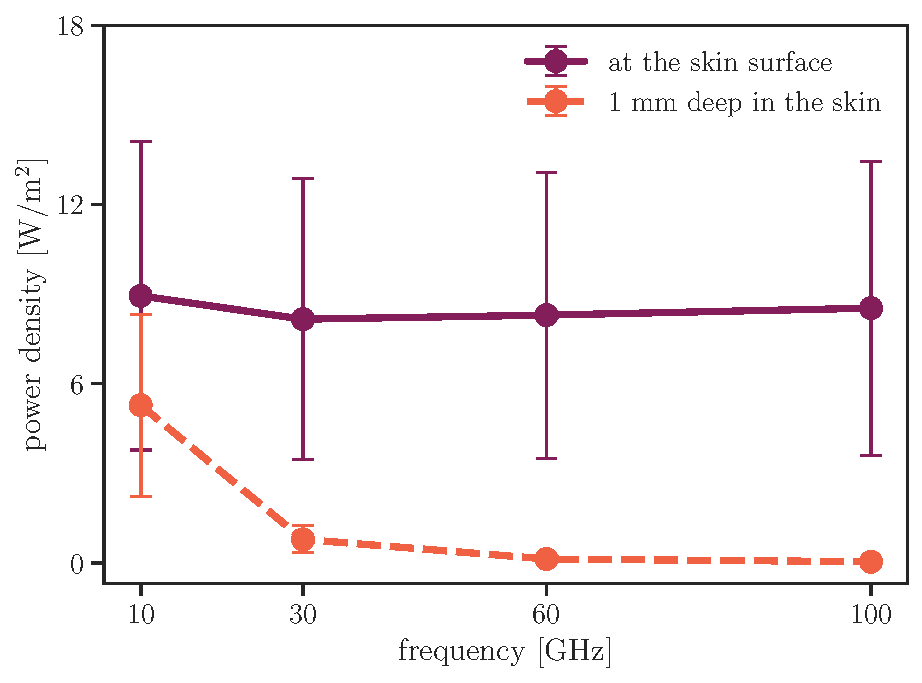
\includegraphics[width=0.8\textwidth]{artwork/pd_decay.pdf}
    \caption{Power density as a function of frequency. At the skin surface (full line), it stays constant with an increase in frequency given the incident power density is bounded between \SI{0}{\watt\per\m\squared} and maximum permissible value as prescribed in~\cite{ICNIRP2020Guidelines,IEEE2019Standard}. At \SI{1}{\mm} depth, power density undergoes steep exponential decay with an increase in frequency.}
    \label{fig:pd_decay}
\end{figure}
With an increase in frequency, for incident power density bounded within the \SI{0}{\watt\per\m\squared} to its maximum permissible value as prescribed in both the \gls{icnirp} guidelines~\cite{ICNIRP2020Guidelines} and \gls{ieee} standard~\cite{IEEE2019Standard}, power density at the surface remains a constant value of about \SI{9}{\watt\per\m\squared}.
But already at a depth of \SI{1}{\mm} perpendicular into the skin, the \gls{apd} drops by \SIlist[list-units=single]{40.98;90.39;98.48;99.59}{\percent}, respectively at \SIlist[list-units=single]{10;30;60;100}{\GHz} considering the corresponding value at the surface.

In the updated version of the \gls{icnirp} guidelines~\cite{ICNIRP2020Guidelines} and \gls{ieee} standard~\cite{IEEE2019Standard}, two definitions of the \gls{apd} are adopted, both derived from the Poynting theorem outlined previously in \cref{eqn:poynting-theorem}.

The first definition of the \gls{apd} is defined as the \gls{tpd}~\cite{Funahashi2018Area-Averaged}
\begin{align}
    \label{eqn:tpd}
    \text{TPD}(x, y) = \int_{z = 0}^{z_\text{max}} \rho(x, y, z) \; \text{SAR}(x, y, z) \; \mathrm{d}z,
\end{align}
spatially-averaged across the exposed surface of tissue, $A$
\begin{align}
    \label{eqn:apd_1}
    S_\text{ab, 1} = \frac{1}{A} \iint_{A} \text{TPD}(x, y) \; \mathrm{d}A,
\end{align}
where the tissue surface is positioned at $z = 0$, and $z_\text{max}$ should be sufficiently larger than the \gls{em} penetration depth.

The second, more rigorous formula is given as the spatially-averaged power density flux on the exposed surface
\begin{equation}
    \label{eqn:apd_2} 
    S_\text{ab, 2} = \frac{1}{2A} \iint_{A} \Re \big[\mathbf{E}(x, y) \times \mathbf{H}^*(x, y) \big] \; \boldsymbol{\hat n} \; \mathrm{d}A
\end{equation}
where $\mathbf{E}$ and $\mathbf{H}$ are the peak values of the complex phasor electric and magnetic field on the surface of the model, respectively, $\Re$ denotes the real part of the vector field, and $*$ is the complex conjugate operator.
Integral variable vector, $\boldsymbol{\hat n} \; \mathrm{d}A$, is set perpendicularly to the exposed surface, where  $\boldsymbol{\hat n}$ corresponds to the unit normal vector to the surface.
Unlike in \cref{eqn:apd_1}, where the \gls{rms} value of the electric field is considered indirectly through expression for \gls{sar} outlined previously in \cref{eqn:sar_3}, the normalization factor of $1/2$ appears as peak values of \gls{em} field components are considered in this definition.

\subsection{Equivalence of Definitions}
In the second definition of the \gls{apd} given in \cref{eqn:apd_2}, the cross product between peak values of the complex phasor electric and magnetic field represents the power density vector field with the direction perpendicular to the plane in which individual components of the \gls{em} field lie, i.e., the Poynting vector.
The surface integral of the normal component of the time-averaged Poynting vector over the exposed region of the tissue is then interpreted as a scalar value, that is, the overall flux passing through that surface.
The divergence theorem, commonly also referred to as the Gauss-Ostrogradsky theorem, relates the flux of a vector field through a closed surface to the divergence of the field in the volume enclosed, or, in other words, it states that the surface integral of a vector field over a closed surface is equal to the volume integral of the divergence over the region inside the surface.
Considering this, both definitions of the \gls{apd} should be equivalent if the surface surrounding a given volume of the tissue is closed, provided there are no active sources in this volume of interest by considering the Poynting theorem outlined in \cref{eqn:poynting-theorem}.

The Poynting vector in \cref{eqn:poynting-theorem,eqn:poynting-theorem-energy,eqn:poynting-vector} is described as the time varying vector field, while in definitions of the \gls{apd}, it is assumed that this vector field is averaged in time and is given in its corresponding phasor notation.
The Poynting vector through the time-harmonic variation can be written as
\begin{align}
    \label{eqn:poynting-vec-time-harmonic}
    \mathcal{P} &= \mathcal{E} \times \mathcal{H} \notag\\
                &= \Re \big[ \mathbf{E} \; \exp{(j \omega t)} \big] \times \Re \big[ \mathbf{H} \; \exp{(j \omega t)} \big] \notag\\
                &= \frac{1}{2} \; \big[ \mathbf{E} \; \exp{(j \omega t)} + \mathbf{E}^*  \; \exp{(-j \omega t)} \big] \times \frac{1}{2} \; \big[ \mathbf{H} \; \exp{(j \omega t)} + \mathbf{H}^*  \; \exp{(-j \omega t)} \big] \notag\\
                &= \frac{1}{2} \; \Re \big[ \mathbf{E} \times \mathbf{H}^* \big] + \frac{1}{2} \; \Re \big[ \mathbf{E} \times \mathbf{H} \; \exp{(2j \omega t)} \big], 
\end{align}
where $t$ is the time domain, and the normalization factor $1/2$ appears as \gls{em} field components are given with their corresponding peak values.
From \cref{eqn:poynting-vec-time-harmonic}, the time-averaged Poynting vector can be written as follows
\begin{align}
    \label{eqn:poynting-vec-time-avg}
    \mathbf{P} = \frac{1}{2} \; \Re \big( \mathbf{E} \times \mathbf{H}^* \big).
\end{align}
Following the above, the time average total power crossing a 2-D surface in 3-D space can then be written as
\begin{align}
    \label{eqn:poynting-flow}
    P_\text{tot} &= \oint_S \mathbf{P} \; \mathrm{d}S \notag\\
                 &= \frac{1}{2} \oint_S \Re \big( \mathbf{E} \times \mathbf{H}^* \big) \; \hat{\boldsymbol{n}} \; \mathrm{d}S,
\end{align}
and it can be additionally averaged across the exposed surface, which, in the case of the closed surface of area $A$, can be written as
\begin{align}
    sP_\text{tot} = \frac{P_\text{tot}}{A}.
\end{align}
Physically, the resulting quantity of the above expression is equivalent to a radiated power density uniformly distributed over the averaging area $A$ and crossing this surface.

Now, by enforcing the divergence theorem onto the Poynting flow given in \cref{eqn:poynting-flow} through any closed surface, $S$, bounding an arbitrary volume, $V$, under the assumption that there are no active sources inside that volume, this expression can be rewritten as~\cite{Poljak2006Advanced}
\begin{align}
    P_\text{tot} &= \frac{1}{2} \iiint_V \nabla \Big [ \Re \big( \mathbf{E} \times \mathbf{H}^* \big) \Big] \; \mathrm{d}V \notag\\
                 &= -\frac{1}{2} \iiint_V \sigma \; |\mathbf{E}|^2 \; \mathrm{d}V.
\end{align}
By separating the total power loss in the expression above into the surface integration of the line integral and, subsequently, averaging it spatially across the surface facing the direction of the impinging \gls{em} wave as
\begin{align}
    \frac{P_\text{tot}}{A}  &= \frac{1}{2A} \iiint_V \sigma \; |\mathbf{E}|^2 \; \mathrm{d}V \notag\\
                            &= \frac{1}{2} \iint_A \int_z \sigma \; |\mathbf{E}|^2 \; \mathrm{dA}\mathrm{d}z,
\end{align}
the above expression perfectly matches the first definition of the \gls{apd} given in \cref{eqn:apd_1}.

Finally, it is clear that the two definitions of the \gls{apd} as given in~\cite{ICNIRP2020Guidelines} are equivalent if the averaging surface for $S_\text{ab, 2}$ is closed and free of sources.
This condition must be met to account for the power deposited within the volume of interest.
This means that $S_\text{ab, 2}$ given as the surface integral of the vector field in  \cref{eqn:apd_2} should take into account the entire closed surface surrounding the exposed volume and not only on the directly exposed, i.e., the front surface facing only the direction of the impinging \gls{em} wave, see \cref{fig:exposed_tissue_volume}.
\begin{figure}[ht]
    \centering
    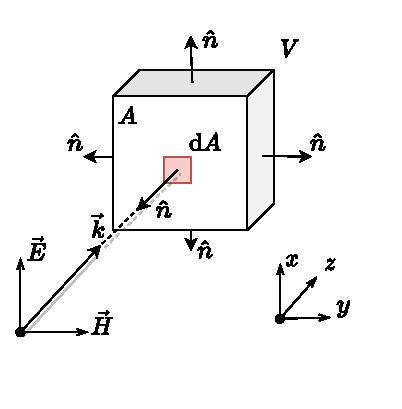
\includegraphics[width=0.46\textwidth]{artwork/exposed_tissue_volume.pdf}
    \caption{Exposed 10-g cubic volume for the assessment of the local exposure to \gls{em} fields.}
    \label{fig:exposed_tissue_volume}
\end{figure}
As this is not the case, it should be expected that $S_\text{ab, 1}$ will always yield values greater than $S_\text{ab, 2}$.
However, since above \SI{6}{\GHz}, power penetration depth is at most about \SI{8}{\mm}, this difference is marginal and thus may be disregarded as the overall contribution of absorption in deeper tissues is less then \SI{10}{\percent} at most.

\section{Incident Power Density}
The \gls{ipd} is used as the \gls{rl} in the \gls{icnirp} guidelines~\cite{ICNIRP2020Guidelines}, that is the \gls{erl} in the \gls{ieee} standard~\cite{IEEE2019Standard}.
It is defined as the modulus of the time-averaged Poynting vector,
\begin{align}
    \label{eqn:ipd}
    S_\text{inc} = |\mathbf{E} \times \mathbf{H}^* |.
\end{align}
In the case of the far-field exposure, it can be simplified to
\begin{align}
    \label{eqn:ipd-far-field}
    S_\text{inc} = \frac{|\mathbf{E}|^2}{Z_0} = |\mathbf{H}|^2 \; Z_0,
\end{align}
where $Z_0$ is the characteristic impedance of free space and it is about \SI{377}{\ohm}.
The above expression is a valid approximation whenever far-field conditions can be assumed which is generally during the assessment of either whole-body exposure or local exposure above \SI{6}{\GHz} if the antenna-to-tissue separation distance is above $\lambda / (2 \pi)$, where $\lambda$ is the wavelength of the incident field.
The said distance of $\lambda / (2 \pi)$ serves well to predict the margin between the reactive and radiative-near field~\cite{Carrasco2019Exposure}.
Because the plane wave reflection coefficient, $\Gamma$, can be used to correlate the incident and absorbed \gls{em} fields only under far-field conditions
\begin{align}
    \label{eqn:ipd-corr}
    S_\text{inc} = \frac{S_\text{ab}}{1 - |\Gamma|^2},
\end{align}
additional considerations are required for the near field.

In the far field, the Poynting vector is purely real, and the direction of the flux does not change in time.
In the near field of an antenna, this is no longer the case as reactive components of the field may contribute to the overall absorption of \gls{em} energy in the exposed body~\cite{Kuster1992Energy}.
Thus, all components of the Poynting vector should be considered to properly assess the \gls{ipd}, and the simple correlation-based formula as outlined in \cref{eqn:ipd-corr} is no longer accurate.

It is generally considered, and prescribed in both the \gls{icnirp} guidelines~\cite{ICNIRP2020Guidelines} and \gls{ieee} standard~\cite{IEEE2019Standard}, that the \gls{rl}/\gls{erl} cannot be used to determine compliance in the reactive near-field region and \gls{br}s/\gls{drl}s should be assessed instead.
However, in the recent \gls{ieee} Guide for the definition of the \gls{ipd} to correlate surface temperature rise~\cite{IEEE2021Guide}, two distinct definitions of the \gls{ipd} have been analyzed.

The first one is directly derived from the second definition of the \gls{apd} -- $S_\text{ab, 2}$ in this document, given in \cref{eqn:apd_2}, and it uses the normal components of the time-averaged Poynting vector in free space as follows
\begin{align}
    \label{eqn:ipd-normal}
    S_\text{inc, n} = \frac{1}{2A} \iint_A \Re \big( \mathbf{E} \times \mathbf{H}^* \big) \; \hat{\boldsymbol{n}} \; \mathrm{d}A,
\end{align}
where $\mathbf{E}$ and $\mathbf{H}$ are peak values of the complex phasor electric and magnetic field in free space, respectively.
The values of the \gls{em} field components are incident, rather than absorbed compared to the definition of the \gls{apd}.

The second definition considers all three components of the Poynting vector field (not solely the normal component) and thus takes into account the norm, i.e., the magnitude, of the power density vector.
It is written as follows
\begin{align}
    \label{eqn:ipd-magnitude}
    S_\text{inc, tot} = \frac{1}{2A} \iint_A \Big | \Re \big( \mathbf{E} \times \mathbf{H}^* \big) \Big | \; \mathrm{d}A.
\end{align}
Both equations for the assessment of the \gls{ipd} given in \cref{eqn:ipd-normal,eqn:ipd-magnitude} are concerning free space without any consideration of the interaction with the human body.
Because, in practice, the averaging area is often not a closed surface, the definition of the \gls{ipd} via the normal component of the Poynting vector may underestimate actual exposure.
Additionally, when the power density is assessed in the near-field region of a radiating source, where the tangential components of the Poynting vector are not negligible compared to its surface-normal components -- reactive-near field at distance $< \frac{\lambda}{2 \pi}$, the definition of the \gls{ipd} via its norm is shown to be slightly better correlated with maximum temperature rise.
However, this has been tested only considering several exposure scenarios in~\cite{IEEE2021Guide} and the overall analysis has shown that the observed difference is marginal and can mainly be attributed to near-field conditions as both definitions correlate well with temperature rise (correlation coefficients > 0.7).